\clearpage
\phantomsection

\setcounter{chapter}{3}
\chapter[{KẾT QUẢ THỰC NGHIỆM VÀ ĐÁNH GIÁ}]{Kết quả thực nghiệm và đánh giá}

Chương này phân tích kết quả thực nghiệm theo bốn nhóm gắn với mục tiêu đề tài: kỹ thuật khám phá, curriculum learning, entropy plateau và observation bottleneck. Mục~\ref{sec:eval_metrics} định nghĩa độ đo và tiêu chí đánh giá trước khi dùng; các mục sau phân tích kết quả theo từng nhóm.

\section{Độ đo và tiêu chí đánh giá}
\label{sec:eval_metrics}

Tất cả chỉ số được trích từ log TensorBoard. Dưới đây là định nghĩa các độ đo chính và tiêu chí dùng để kết luận:

\begin{itemize}
    \item \textbf{cumulative\_reward}: tổng phần thưởng tích lũy mỗi episode theo thang phần thưởng đang dùng (v1 hoặc v2). \textit{Chú ý}: run55 dùng v2 nên không so sánh trực tiếp với các run v1.
    \item \textbf{clear\_rate}: tỷ lệ episode tác nhân tiêu diệt toàn bộ kẻ địch trong phòng. Tiêu chí thành công: clear\_rate $\geq 0.5$. Đây là độ đo trực tiếp nhất cho mục tiêu chiến đấu của đề tài.
    \item \textbf{kills/episode}: số kẻ địch trung bình bị tiêu diệt mỗi episode. Bổ sung cho clear\_rate khi phòng có nhiều kẻ địch.
    \item \textbf{entropy (nat)}: độ hỗn loạn của phân phối hành động. Giá trị cao = chính sách chưa quyết đoán; max lý thuyết = $\ln(3)+\ln(3)+\ln(3)+\ln(9) \approx 5.49$ nat. Tiêu chí plateau: entropy bão hòa nhất quán ở 4.40 nat trên nhiều cấu hình là dấu hiệu nút thắt không phải từ thuật toán.
    \item \textbf{tail-50}: trung bình 50 episode cuối để tránh so sánh giá trị đỉnh. Tất cả chỉ số so sánh trong chương này đều dùng tail-50 trừ khi ghi chú khác.
    \item \textbf{rolling\_reward\_200k}: phần thưởng trung bình trượt cửa sổ 200k bước, dùng để vẽ xu hướng học.
    \item \textbf{reward\_hard\_from\_140k}: phần thưởng trung bình sau khi curriculum đã chuyển vào Hard (từ bước $\sim$140k), dùng để so sánh công bằng giữa các run curriculum.
\end{itemize}

\textit{Hạn chế so sánh}: run34--run42 dừng ở 1.0M bước; run46+ chạy đến 3.0M bước. So sánh liên nhóm là so sánh giữa cấu hình hoàn chỉnh, không phải tại cùng số bước.

\begin{table}[H]
    \centering
    \scriptsize
    \setlength{\tabcolsep}{4pt}
    \renewcommand{\arraystretch}{1.15}
    \caption{Các chỉ số hành vi chính ở cuối quá trình huấn luyện}
    \label{tab:run_metrics_main}
    \begin{tabular}{l p{3.0cm} c c c c c c c c}
        \toprule
        \textbf{Run} & \textbf{Thiết lập} & \textbf{Step} & \textbf{Reward} & \textbf{Clear} & \textbf{Kills} & \textbf{Dmg+} & \textbf{Dmg-} & \textbf{Dash+} & \textbf{Ent} \\
        \midrule
        run34 & PPO baseline & 1.00M & 2.073 & 0.129 & 0.721 & 25.977 & 16.867 & 0.149 & 4.408 \\
        run35 & PPO + ICM & 1.00M & 2.416 & 0.173 & 0.752 & 26.614 & 15.242 & 0.116 & 4.407 \\
        run36 & PPO + RND & 1.00M & 2.487 & 0.159 & 0.796 & 28.068 & 14.013 & 0.107 & 4.406 \\
        run42 & PPO + LSTM & 1.00M & 2.411 & 0.163 & 0.769 & 27.140 & 15.775 & 0.132 & 4.405 \\
        run46 & PPO + Curriculum & 3.00M & 3.843 & 0.267 & 0.994 & 35.135 & 19.368 & 0.245 & 4.409 \\
        run47 & Curriculum + LSTM & 3.00M & 3.765 & 0.241 & 0.921 & 32.884 & 16.420 & 0.228 & 4.405 \\
        run50 & Curriculum + ICM & 3.00M & 4.369 & 0.273 & 1.016 & 36.161 & 23.132 & 0.334 & 4.411 \\
        run54 & 4-tier fixed-to-random & 3.00M & 3.925 & 0.242 & 0.945 & 33.673 & 17.966 & 0.179 & 4.407 \\
        run55 & Curriculum + reward v2 & 3.00M & 9.337 & 0.267 & 1.014 & 35.685 & 21.312 & 0.240 & 4.407 \\
        run62 & LocalGrid + Aggressive + ICM + 4-tier & 33.45M & 14.105 & 0.626 & 1.530 & 47.780 & 25.501 & 0.400 & 3.099 \\
        \bottomrule
    \end{tabular}
    \vspace{4pt}
    \begin{minipage}{0.96\textwidth}
        \small\textit{Ghi chú}: run62 không so sánh trực tiếp với các run khác do khác biệt về kích thước quan sát (432 chiều so với 207), số bước huấn luyện (33.45M so với 1--3M bước), hyperparameter PPO điều chỉnh và các thay đổi môi trường bổ sung. Run62 được đưa vào bảng để tham khảo, không phải để so sánh ngang hàng.
    \end{minipage}
\end{table}

\begin{table}[H]
    \centering
    \scriptsize
    \setlength{\tabcolsep}{5pt}
    \renewcommand{\arraystretch}{1.15}
    \caption{Các chỉ số loss, chính sách và phần thưởng nội tại}
    \label{tab:run_metrics_aux}
    \begin{tabular}{l p{3.5cm} c c c c c c}
        \toprule
        \textbf{Run} & \textbf{Thiết lập} & \textbf{P-loss} & \textbf{V-loss} & \textbf{V-est} & \textbf{Dash/dec} & \textbf{ICM inv.} & \textbf{Int. rew.} \\
        \midrule
        run34 & PPO baseline & 0.016 & 0.140 & 0.170 & 0.0002 & -- & -- \\
        run35 & PPO + ICM & 0.017 & 0.072 & 0.169 & 0.0002 & 4.360 & 0.150 \\
        run36 & PPO + RND & 0.016 & 0.071 & 0.167 & 0.0002 & -- & 0.099 \\
        run42 & PPO + LSTM & 0.082 & 0.168 & 0.178 & 0.0002 & -- & -- \\
        run46 & PPO + Curriculum & 0.017 & 0.207 & 0.401 & 0.0005 & -- & -- \\
        run47 & Curriculum + LSTM & 0.079 & 0.229 & 0.380 & 0.0004 & -- & -- \\
        run50 & Curriculum + ICM & 0.016 & 0.113 & 0.483 & 0.0011 & 4.337 & 0.185 \\
        run54 & 4-tier fixed-to-random & 0.017 & 0.200 & 0.416 & 0.0005 & -- & -- \\
        run55 & Curriculum + reward v2 & 0.016 & 0.662 & 0.962 & 0.0005 & -- & -- \\
        run62 & LocalGrid + Aggressive + ICM + 4-tier & 0.017 & 0.227 & 2.455 & -- & -- & -- \\
        \bottomrule
    \end{tabular}
\end{table}

Trong Bảng~\ref{tab:run_metrics_main}, cột Reward là \texttt{reward\_tail50} với các run không curriculum và \texttt{reward\_hard\_from\_140k} với các run curriculum; các cột Clear, Kills, Dmg+/Dmg-, Dash+ và Ent lần lượt là \texttt{cleared\_tail50}, \texttt{kills\_tail50}, \texttt{damage\_dealt/taken\_tail50}, \texttt{useful\_dash\_rate\_tail50} và \texttt{entropy\_tail50}. Bảng~\ref{tab:run_metrics_aux} giữ các tín hiệu chẩn đoán quan trọng: policy loss, value loss, ước lượng giá trị ngoại tại, tần suất dash, inverse loss của ICM và phần thưởng nội tại. Các cột trống được ký hiệu ``--'' vì run tương ứng không sử dụng kỹ thuật đó.

\begin{figure}[H]
    \centering
    
\includegraphics[width=0.98\textwidth]{figures/training/training_reward_curves.png}
    \caption{Đường phần thưởng trong quá trình huấn luyện của các cấu hình chính}
    \label{fig:training_reward_curves}
\end{figure}

Các run không dùng curriculum kết thúc ở 1M bước nên được giữ phẳng sau mốc này để thuận tiện so sánh trực quan trên cùng một trục thời gian. Riêng run55 sử dụng reward v2, do đó giá trị phần thưởng tuyệt đối của run này không được so trực tiếp với các run dùng reward v1; hình chủ yếu dùng để đọc xu hướng học và vị trí tương đối giữa các nhóm thí nghiệm.

\section{Kỹ thuật khám phá có giúp ích không?}
\label{sec:exploration_techniques}

Run34 là cấu hình PPO baseline, chưa áp dụng curriculum learning. Sau 1 triệu bước huấn luyện, phần thưởng tích lũy trung bình trên 50 episode cuối đạt 2.073, tỷ lệ dọn phòng trung bình đạt 0.129 và tỷ lệ dọn phòng cao nhất đạt 0.50. Kết quả này cho thấy tác nhân đã học được một số hành vi cơ bản như tiếp cận và tấn công kẻ địch, nhưng chưa duy trì ổn định khả năng dọn phòng trên phân phối bản đồ khó.

Hai biến thể phần thưởng nội tại được đánh giá là ICM ở run35 và RND ở run36. ICM đạt phần thưởng tail-50 là 2.416, RND đạt 2.487. Cả hai đều cải thiện so với PPO baseline, nhưng mức tăng còn tương đối nhỏ và chưa tạo ra thay đổi bản chất trong hành vi của tác nhân. Có thể thấy khó khăn chính của môi trường không chỉ nằm ở việc thiếu tín hiệu thúc đẩy khám phá, mà còn đến từ độ khó ban đầu của phân phối bản đồ và nhiệm vụ chiến đấu.

\begin{figure}[H]
    \centering
    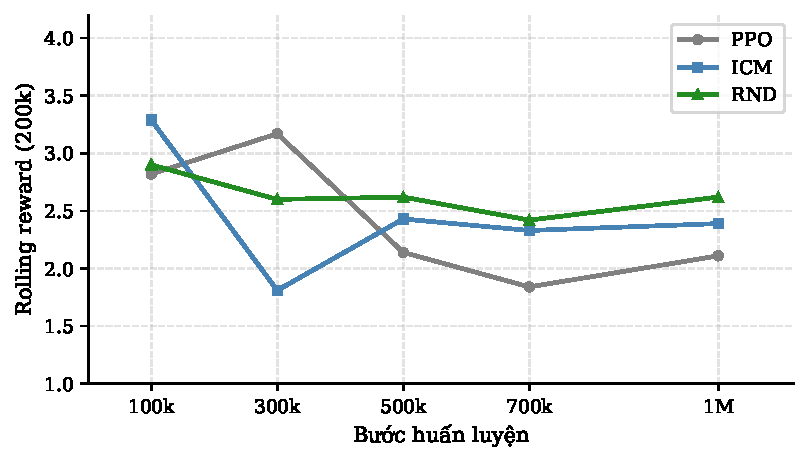
\includegraphics[width=0.85\textwidth]{figures/training/fig42_reward_ppo_icm_rnd.pdf}
    \caption{Phần thưởng trung bình trượt 200k bước của PPO baseline, ICM và RND trong 1M bước đầu}
    \label{fig:baseline_intrinsic_reward}
\end{figure}

\subsection{ICM và dấu hiệu biểu diễn chưa ổn định}

ICM học một inverse model dự đoán hành động từ trạng thái trước và sau \cite{Pathak2017}. Với action space $(3,3,3,9)$, entropy ngẫu nhiên lý thuyết là khoảng 5.49 nat. Inverse loss của run35 quanh 4.36, chỉ giảm khoảng 21\% so với mức ngẫu nhiên lý thuyết. Điều này cho thấy biểu diễn học được còn yếu: biểu diễn không phân biệt tốt tác động của từng nhánh hành động trong môi trường nhiều yếu tố nhiễu như đạn, kẻ địch và bản đồ sinh theo thủ tục.

\begin{figure}[H]
    \centering
    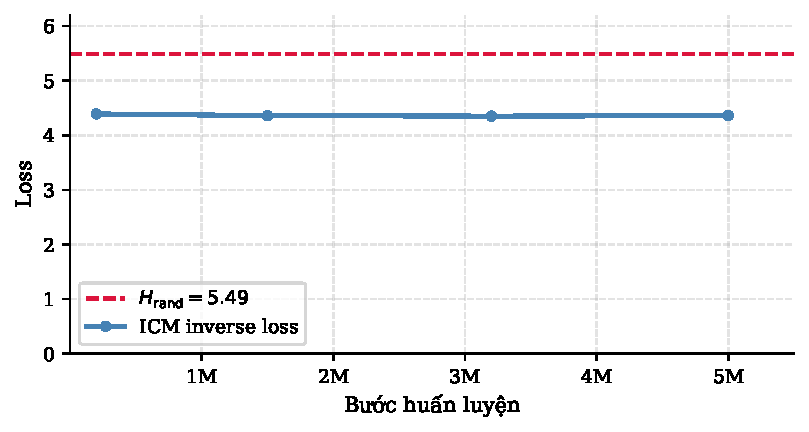
\includegraphics[width=0.85\textwidth]{figures/training/fig43_icm_inverse_loss.pdf}
    \caption{Inverse loss của ICM duy trì gần mức ngẫu nhiên lý thuyết}
    \label{fig:icm_inverse_plateau}
\end{figure}

RND không cần dự đoán hành động nên tránh được hiện tượng inverse loss suy giảm chất lượng \cite{Burda2018}, nhưng phần thưởng nội tại của run36 giảm nhanh về mức nhỏ khi mô hình dự đoán quen với phân phối quan sát. Vì vậy, RND tốt hơn ICM một chút ở phần thưởng tail-50, nhưng vẫn chưa vượt mốc so sánh đáng kể.

\section{LSTM: bộ nhớ có cần thiết không?}

Run42 thêm LSTM với bộ nhớ kích thước 256 và chuỗi quan sát dài 64 bước. Khác với ICM/RND, LSTM có xu hướng học chậm nhưng tăng dần về cuối. Phần thưởng trung bình trượt 200k bước tăng từ 1.64 ở mốc 100k lên 2.71 ở mốc 1M. Xu hướng này phù hợp với giả thuyết bộ nhớ có ích cho hồi chiêu, đạn và trạng thái khuất tầm nhìn; tuy nhiên lợi ích chưa đủ lớn để tạo cải thiện đáng chú ý trong quy mô huấn luyện hiện tại.

\begin{figure}[H]
    \centering
    
\includegraphics[width=0.85\textwidth]{figures/training/fig44_lstm_trend.pdf}
    \caption{Run42 LSTM-only có xu hướng tăng dần nhưng vẫn quanh mức của các run dùng phần thưởng nội tại}
    \label{fig:lstm_trend}
\end{figure}

Như vậy, kiến trúc bộ nhớ có thể là hướng cải tiến phụ chứ không giải quyết được vấn đề chính của môi trường: tác nhân vẫn bắt đầu từ phân phối Hard quá rộng và khó nhận được chuỗi phần thưởng thành công đủ thường xuyên.

\section{Curriculum learning: cải thiện nổi bật}

Run46 là thí nghiệm quan trọng nhất. Curriculum bắt đầu ở Easy, chuyển sang Medium tại khoảng 70k bước và chuyển sang Hard tại khoảng 140k bước. Sau khi vào Hard, phần thưởng trung bình đạt 3.843, cao hơn 85\% so với mốc so sánh tail-50 2.073:

\begin{equation}
    \frac{3.843 - 2.073}{2.073} \approx 85\%.
\end{equation}

\begin{figure}[H]
    \centering
    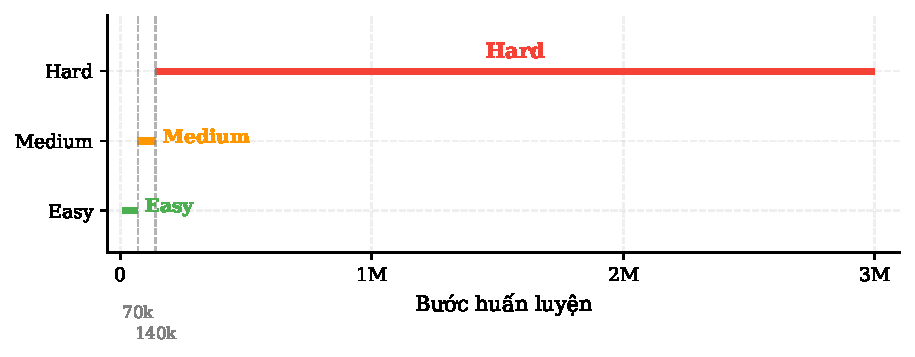
\includegraphics[width=0.85\textwidth]{figures/training/fig45_run46_lesson_transition.pdf}
    \caption{Lesson transition của run46: Easy $\rightarrow$ Medium $\rightarrow$ Hard}
    \label{fig:run46_lesson_transition}
\end{figure}

Phần thưởng theo lesson của run46 cho thấy trung bình ở Easy đạt 6.364, ở Medium đạt 4.181 và ở Hard đạt 3.843. Khi vào Hard, đường phần thưởng không tăng tuyến tính mà dao động trong vùng 3.1--4.2 theo cửa sổ trượt 200k bước. Dao động này là hợp lý vì nhóm Hard có nhiều cấu hình bản đồ hơn, đồng thời vị trí sinh và phân phối kẻ địch cũng đa dạng hơn.

\begin{figure}[H]
    \centering
    
\includegraphics[width=0.98\textwidth]{figures/training/curriculum_reward_trend.png}
    \caption{Xu hướng phần thưởng trong các run curriculum}
    \label{fig:curriculum_reward_trend}
    \vspace{0.2em}
    \begin{minipage}{0.94\textwidth}
        \small
        Hình cho thấy phần thưởng không tăng đều sau khi vào Hard mà dao động quanh một vùng ổn định. Run50 cao hơn run46 ở phần sau quá trình huấn luyện -- ICM chỉ phát huy rõ khi chính sách đã có kỹ năng cơ bản từ curriculum.
    \end{minipage}
\end{figure}

\begin{figure}[H]
    \centering
    
\includegraphics[width=0.98\textwidth]{figures/training/curriculum_clear_rate_trend.png}
    \caption{Xu hướng tỷ lệ dọn phòng trong các run curriculum}
    \label{fig:curriculum_clear_rate_trend}
    \vspace{0.2em}
    \begin{minipage}{0.94\textwidth}
        \small
        Tỷ lệ dọn phòng tăng mạnh ở giai đoạn đầu rồi chững lại khi bài toán chuyển sang phân phối Hard. Vì tỷ lệ dọn phòng là chỉ số kết quả, đường cong này bổ sung cho phần thưởng: cải thiện không chỉ nằm ở phần thưởng định hình mà còn ở hành vi dọn phòng thực tế.
    \end{minipage}
\end{figure}

\begin{figure}[H]
    \centering
    
\includegraphics[width=\textwidth]{figures/training/curriculum_entropy_trend.png}
    \caption{Xu hướng entropy chính sách trong các run curriculum}
    \label{fig:curriculum_entropy_trend}
    \vspace{0.2em}
    \begin{minipage}{0.94\textwidth}
        \small
        Entropy của ba run nhanh chóng rơi về vùng xấp xỉ 4.40 nat và gần như đi ngang. Điều này giải thích vì sao tăng phần thưởng/tỷ lệ dọn phòng không đồng nghĩa với việc chính sách trở nên quyết định hơn đáng kể.
    \end{minipage}
\end{figure}

\begin{figure}[H]
    \centering
    
\includegraphics[width=\textwidth]{figures/training/curriculum_lesson_schedule.png}
    \caption{Lịch chuyển lesson trong các run curriculum}
    \label{fig:curriculum_lesson_schedule}
    \vspace{0.2em}
    \begin{minipage}{0.94\textwidth}
        \small
        Run46 và run50 chuyển lên Hard từ rất sớm nên phần lớn 3M bước vẫn đánh giá trên cùng phân phối khó. Run54 có thêm lesson Hard Random, nên đường lesson đạt mức 3 và phản ánh biến thể fixed-to-random spawn.
    \end{minipage}
\end{figure}

Trong các run đã thực hiện, đây là xu hướng mạnh nhất của khóa luận: curriculum không chỉ tăng phần thưởng trung bình mà còn cải thiện các chỉ số hành vi. Tail-50 của run46 đạt 0.994 kills/episode và tỷ lệ dọn phòng tail-50 đạt 0.267, cao hơn rõ rệt so với mốc so sánh. Về mặt cơ chế, curriculum learning hỗ trợ tín hiệu học theo từng giai đoạn: ở Easy, tác nhân gặp các episode thành công đủ thường xuyên để học chuỗi tiếp cận -- ngắm -- tấn công; khi sang Medium và Hard, chính sách đã có kỹ năng cơ bản thay vì khám phá từ gần như ngẫu nhiên. Do mỗi cấu hình mới chỉ có một seed, kết luận này cần được xác nhận thêm bằng các run lặp lại có error bar.

\section{Kết hợp curriculum với LSTM và ICM}

Run47 thêm LSTM vào curriculum. Trung bình ở Hard đạt 3.765, thấp hơn nhẹ so với 3.843 của run46. Chênh lệch này nhỏ, chưa đủ để kết luận LSTM làm xấu chính sách, nhưng đủ cho thấy bộ nhớ không tạo thêm cải thiện rõ ràng khi curriculum đã cung cấp nền tảng để khám phá.

Có hai giả thuyết giải thích kết quả này. Giả thuyết đầu tiên là \textit{LSTM làm chậm tốc độ hội tụ của PPO}: policy loss của run47 đạt 0.079, cao hơn gần 5 lần so với 0.017 của run46. Các trọng số hồi tiếp của LSTM cần nhiều mẫu hơn để ổn định, làm cập nhật chính sách kém hiệu quả trong cùng 3M bước. Giả thuyết còn lại là \textit{curriculum đã giải quyết phần lớn nhu cầu về bộ nhớ}: trong môi trường thưa thưởng, lợi ích chính của LSTM là giúp tác nhân nhớ chuỗi hành vi thành công trong episode dài; khi curriculum đã thu hẹp phân phối bản đồ về Easy/Medium ở giai đoạn đầu, độ dài hiệu quả của chuỗi quyết định ngắn lại, làm giảm lợi thế tương đối của LSTM so với MLP thuần.

Run50 bổ sung ICM trên nền curriculum và được huấn luyện đủ 3.00M bước. Trên vùng Hard, phần thưởng trung bình đạt 4.369, cao hơn run46 (3.843); tail-50 cuối run đạt 4.707. Một số chỉ số hành vi cũng cải thiện nhẹ: số kẻ địch tiêu diệt trung bình 1.016, tỷ lệ dọn phòng tail-50 0.273 và tỷ lệ dash hữu ích 0.334. ICM do đó có thể hỗ trợ tác nhân khám phá thêm các hành vi có ích một khi đã được curriculum dẫn qua giai đoạn học ban đầu. Tuy nhiên, inverse loss vẫn ở mức cao, khoảng 4.337, chỉ giảm nhẹ so với run35. Như vậy, cải thiện của run50 chủ yếu thể hiện ở hành vi và phần thưởng. Vấn đề biểu diễn phát sinh từ không gian hành động rời rạc nhiều nhánh chưa được ICM giải quyết triệt để.

\begin{table}[H]
    \centering
    \small
    \caption{So sánh các \emph{stacking test} với curriculum baseline}
    \label{tab:stacking_tests}
    \begin{tabular}{|p{4.4cm}|c|c|p{4.8cm}|}
        \hline
        \textbf{Run} & \textbf{Steps log} & \textbf{Phần thưởng trung bình ở Hard} & \textbf{Nhận xét} \\
        \hline
        run46 Curriculum & 3.0M & 3.843 & Baseline curriculum, cải thiện chính. \\
        \hline
        run47 Curriculum + LSTM & 3.0M & 3.765 & Gần tương đương, không có tác dụng bổ trợ rõ. \\
        \hline
        run50 Curriculum + ICM & 3.0M & 4.369 & Cải thiện phần thưởng và số lần tiêu diệt so với run46; inverse loss vẫn cao. \\
        \hline
    \end{tabular}
\end{table}

Kết quả cập nhật này làm kết luận tinh tế hơn: curriculum vẫn là yếu tố nền quan trọng nhất, còn ICM có thể tạo thêm lợi ích khi tác nhân đã có kỹ năng cơ bản từ các lesson dễ hơn. Tuy vậy, inverse loss vẫn ở mức cao -- tín hiệu nội tại chủ yếu hỗ trợ khám phá/hành vi ở mức thực nghiệm, chưa chứng minh rằng biểu diễn của ICM đã học tốt quan hệ hành động--chuyển trạng thái trong môi trường này.

\section{Giảm phương sai: vị trí sinh cố định rồi ngẫu nhiên}

Run54 mở rộng curriculum thành 4 lesson: \emph{Easy Fixed}, \emph{Medium Fixed}, \emph{Hard Fixed} và \emph{Hard Random}. Lesson \emph{Hard Random} bắt đầu khoảng 280k bước. Phần thưởng trung bình ở Hard đạt 3.925, số lần tiêu diệt cuối run đạt 0.945 và sát thương gây ra đạt 33.673. Các chỉ số này gần run46 nhưng không vượt rõ, nên kết quả này được xem là tương đương với mức cải thiện nhỏ.

\begin{figure}[H]
    \centering
    
\includegraphics[width=0.85\textwidth]{figures/training/fig410_run54_four_tier.pdf}
    \caption{Curriculum 4 bậc của run54: vị trí sinh cố định trước, vị trí sinh ngẫu nhiên sau}
    \label{fig:run54_four_tier}
\end{figure}

Vị trí sinh cố định giúp giảm phương sai ở giai đoạn đầu, nhưng khi chuyển sang Hard Random thì tác nhân vẫn phải xử lý cùng phân phối khó. Vì vậy, run54 chỉ cải thiện nhẹ ở hành vi chiến đấu và không làm thay đổi xu hướng tổng quát: curriculum là yếu tố chính trong nhóm thí nghiệm này, còn chuyển từ vị trí sinh cố định sang ngẫu nhiên là một biến thể thiết kế môi trường có tác động nhỏ hơn so với chính curriculum.

\section{Reward v2: tăng phần thưởng kết quả nhưng thay đổi thang đo}

Run55 thay đổi cấu trúc hàm thưởng: tăng mạnh phần thưởng tiêu diệt/dọn phòng/sát thương/tấn công đúng hướng, giảm phần thưởng tiếp cận và phạt mạnh hơn hành vi đứng gần địch không hành động. Run được huấn luyện đến 3.00M bước. Phần thưởng tail-50 đạt 9.600 và trung bình ở Hard đạt 9.337, nhưng không thể so sánh trực tiếp với run46 vì thang thưởng đã thay đổi.

Chỉ số đáng chú ý hơn là đỉnh tỷ lệ dọn phòng đạt 0.80, cao hơn đỉnh 0.615 của run46. Khi nhấn mạnh kết quả, reward v2 đẩy tác nhân tấn công quyết đoán hơn. Tuy nhiên entropy tail vẫn quanh 4.408 -- reward v2 chưa phá được entropy plateau.

Do đó, run55 được tách khỏi nhóm so sánh reward v1 khi diễn giải phần thưởng trung bình. Với reward v2, các chỉ số đáng dùng hơn là tỷ lệ dọn phòng, số kẻ địch tiêu diệt, sát thương gây ra, sát thương nhận vào, tỷ lệ sống sót hoặc các chỉ số đã chuẩn hóa theo cùng thang đo. Cách tách này tránh hiểu nhầm rằng giá trị phần thưởng 9.337 của run55 có thể so trực tiếp với 3.843 của run46.

\begin{figure}[H]
    \centering
    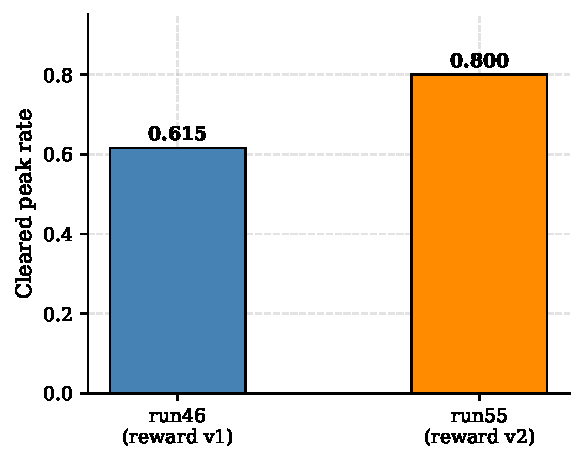
\includegraphics[width=0.55\textwidth]{figures/training/fig411_reward_v2_clear_peak.pdf}
    \caption{Run55 tăng đỉnh tỷ lệ dọn phòng, nhưng phần thưởng trung bình không so trực tiếp do đổi thang thưởng}
    \label{fig:reward_v2_clear_peak}
\end{figure}

\section{Entropy plateau: hiện tượng và nguyên nhân}

Một hiện tượng nhất quán xuyên suốt các run là entropy của chính sách gần như không giảm khỏi vùng 4.40 nat. Với entropy cực đại lý thuyết $H_{\max}\approx 5.49$ nat ở phương trình~\ref{eq:max_entropy}, mức 4.40 tương đương khoảng 80\% của cực đại. Do action mask có thể làm cực đại thực tế thấp hơn, không nên diễn giải đây là chính sách hoàn toàn ngẫu nhiên; tuy vậy, chính sách vẫn giữ mức ngẫu nhiên cao.

\begin{figure}[H]
    \centering
    
\includegraphics[width=0.95\textwidth]{figures/training/fig412_entropy_plateau.pdf}
    \caption{Entropy tail-50 của các run chính. Cấu hình run62 (33.45M bước, kết hợp lưới cục bộ, curriculum 4 bậc và ICM) phá vỡ plateau 4.40 nat.}
    \label{fig:entropy_plateau}
\end{figure}

Trong các ablation chính giữ nguyên quan sát 207 chiều, plateau này không được giải quyết bởi ICM, RND, LSTM, curriculum learning, giảm phương sai vị trí sinh hay thiết kế lại phần thưởng. Khi run62 kết hợp quan sát lưới cục bộ với curriculum 4 bậc, ICM và được huấn luyện đến 33.45M bước, entropy giảm bền vững xuống 3.10 nat và duy trì ở mức này. Kết luận thận trọng được cập nhật như sau: plateau xuất phát chủ yếu từ biểu diễn quan sát 207 chiều và số bước huấn luyện 1--3M trong các ablation chính, không phải từ giới hạn cứng của PPO hay action space hiện tại.

\section{Tổng hợp kết quả}

\begin{table}[H]
    \centering
    \scriptsize
    \setlength{\tabcolsep}{3pt}
    \renewcommand{\arraystretch}{1.18}
    \caption{Tổng hợp các run chính}
    \label{tab:master_ablation}
    \begin{tabular}{|>{\raggedright\arraybackslash}p{1.15cm}|>{\raggedright\arraybackslash}p{2.65cm}|>{\centering\arraybackslash}p{1.05cm}|>{\centering\arraybackslash}p{1.95cm}|>{\centering\arraybackslash}p{1.35cm}|>{\raggedright\arraybackslash}p{4.65cm}|}
        \hline
        \textbf{Run} & \textbf{Thiết lập} & \textbf{Steps} & \textbf{Reward} & \textbf{Kills} & \textbf{Kết luận} \\
        \hline
        run34 & PPO baseline & 1.0M & 2.073 & 0.721 & Mốc so sánh; học được chiến đấu cơ bản nhưng đạt trần ở mức thấp. \\
        \hline
        run35 & PPO + ICM & 1.0M & 2.416 & 0.752 & Cải thiện nhỏ; inverse loss cao. \\
        \hline
        run36 & PPO + RND & 1.0M & 2.487 & 0.796 & Tốt hơn ICM nhẹ, nhưng chưa tạo cải thiện đáng chú ý. \\
        \hline
        run42 & PPO + LSTM & 1.0M & 2.411 & 0.769 & Học chậm nhưng tăng dần; lợi ích hạn chế. \\
        \hline
        run46 & PPO + Curriculum & 3.0M & 3.843 & 0.994 & Cải thiện chính, kill/episode và tỷ lệ dọn phòng đều tăng rõ. \\
        \hline
        run47 & Curriculum + LSTM & 3.0M & 3.765 & 0.921 & Không tạo tác dụng bổ trợ rõ với curriculum. \\
        \hline
        run50 & Curriculum + ICM & 3.0M & 4.369 & 1.016 & Bổ trợ nhẹ với curriculum; inverse loss vẫn cao. \\
        \hline
        run54 & 4-tier fixed-to-random & 3.0M & 3.925 & 0.945 & Tương đương run46; fixed-to-random chỉ cải thiện nhẹ. \\
        \hline
        run55 & Curriculum + reward v2 & 3.0M & 9.337 & 1.014 & Đỉnh tỷ lệ dọn phòng cao hơn; thang thưởng khác nên không so trung bình trực tiếp. \\
        \hline
        run62 & LocalGrid + Aggressive + ICM + 4-tier & 33.45M & 14.105 & 1.530 & Entropy 3.10 -- plateau bị phá vỡ; tỷ lệ dọn phòng 0.626; tiệm cận BFS mà không cài cứng. \\
        \hline
    \end{tabular}
\end{table}

Một lưu ý quan trọng khi đọc Bảng~\ref{tab:master_ablation} là quy mô huấn luyện giữa các nhóm chưa hoàn toàn đồng nhất. Các run không dùng curriculum như run34, run35, run36 và run42 kết thúc ở 1.0M bước, trong khi các run curriculum chính được huấn luyện đến 3.0M bước. Vì vậy, so sánh giữa hai nhóm phản ánh xu hướng thực nghiệm của toàn bộ cấu hình huấn luyện, nhưng chưa tách biệt hoàn toàn ảnh hưởng của curriculum khỏi ảnh hưởng của số bước huấn luyện nhiều hơn. Để so sánh chặt chẽ hơn, các baseline/ICM/RND/LSTM cần được huấn luyện đến 3.0M bước, hoặc các run curriculum cần được báo cáo thêm tại cùng mốc 1.0M bước.

\begin{figure}[H]
\centering

\includegraphics[width=0.9\textwidth]{figures/training/fig413_reward_comparison.pdf}
\caption{So sánh phần thưởng trung bình giữa các run dùng reward v1. Đường nét đứt ở 2.07 là mức mốc so sánh. Run55 (reward v2, trung bình 9.337) có thang thưởng khác nên không đưa vào biểu đồ.}
\label{fig:reward_comparison_all}
\end{figure}

\begin{figure}[H]
    \centering
    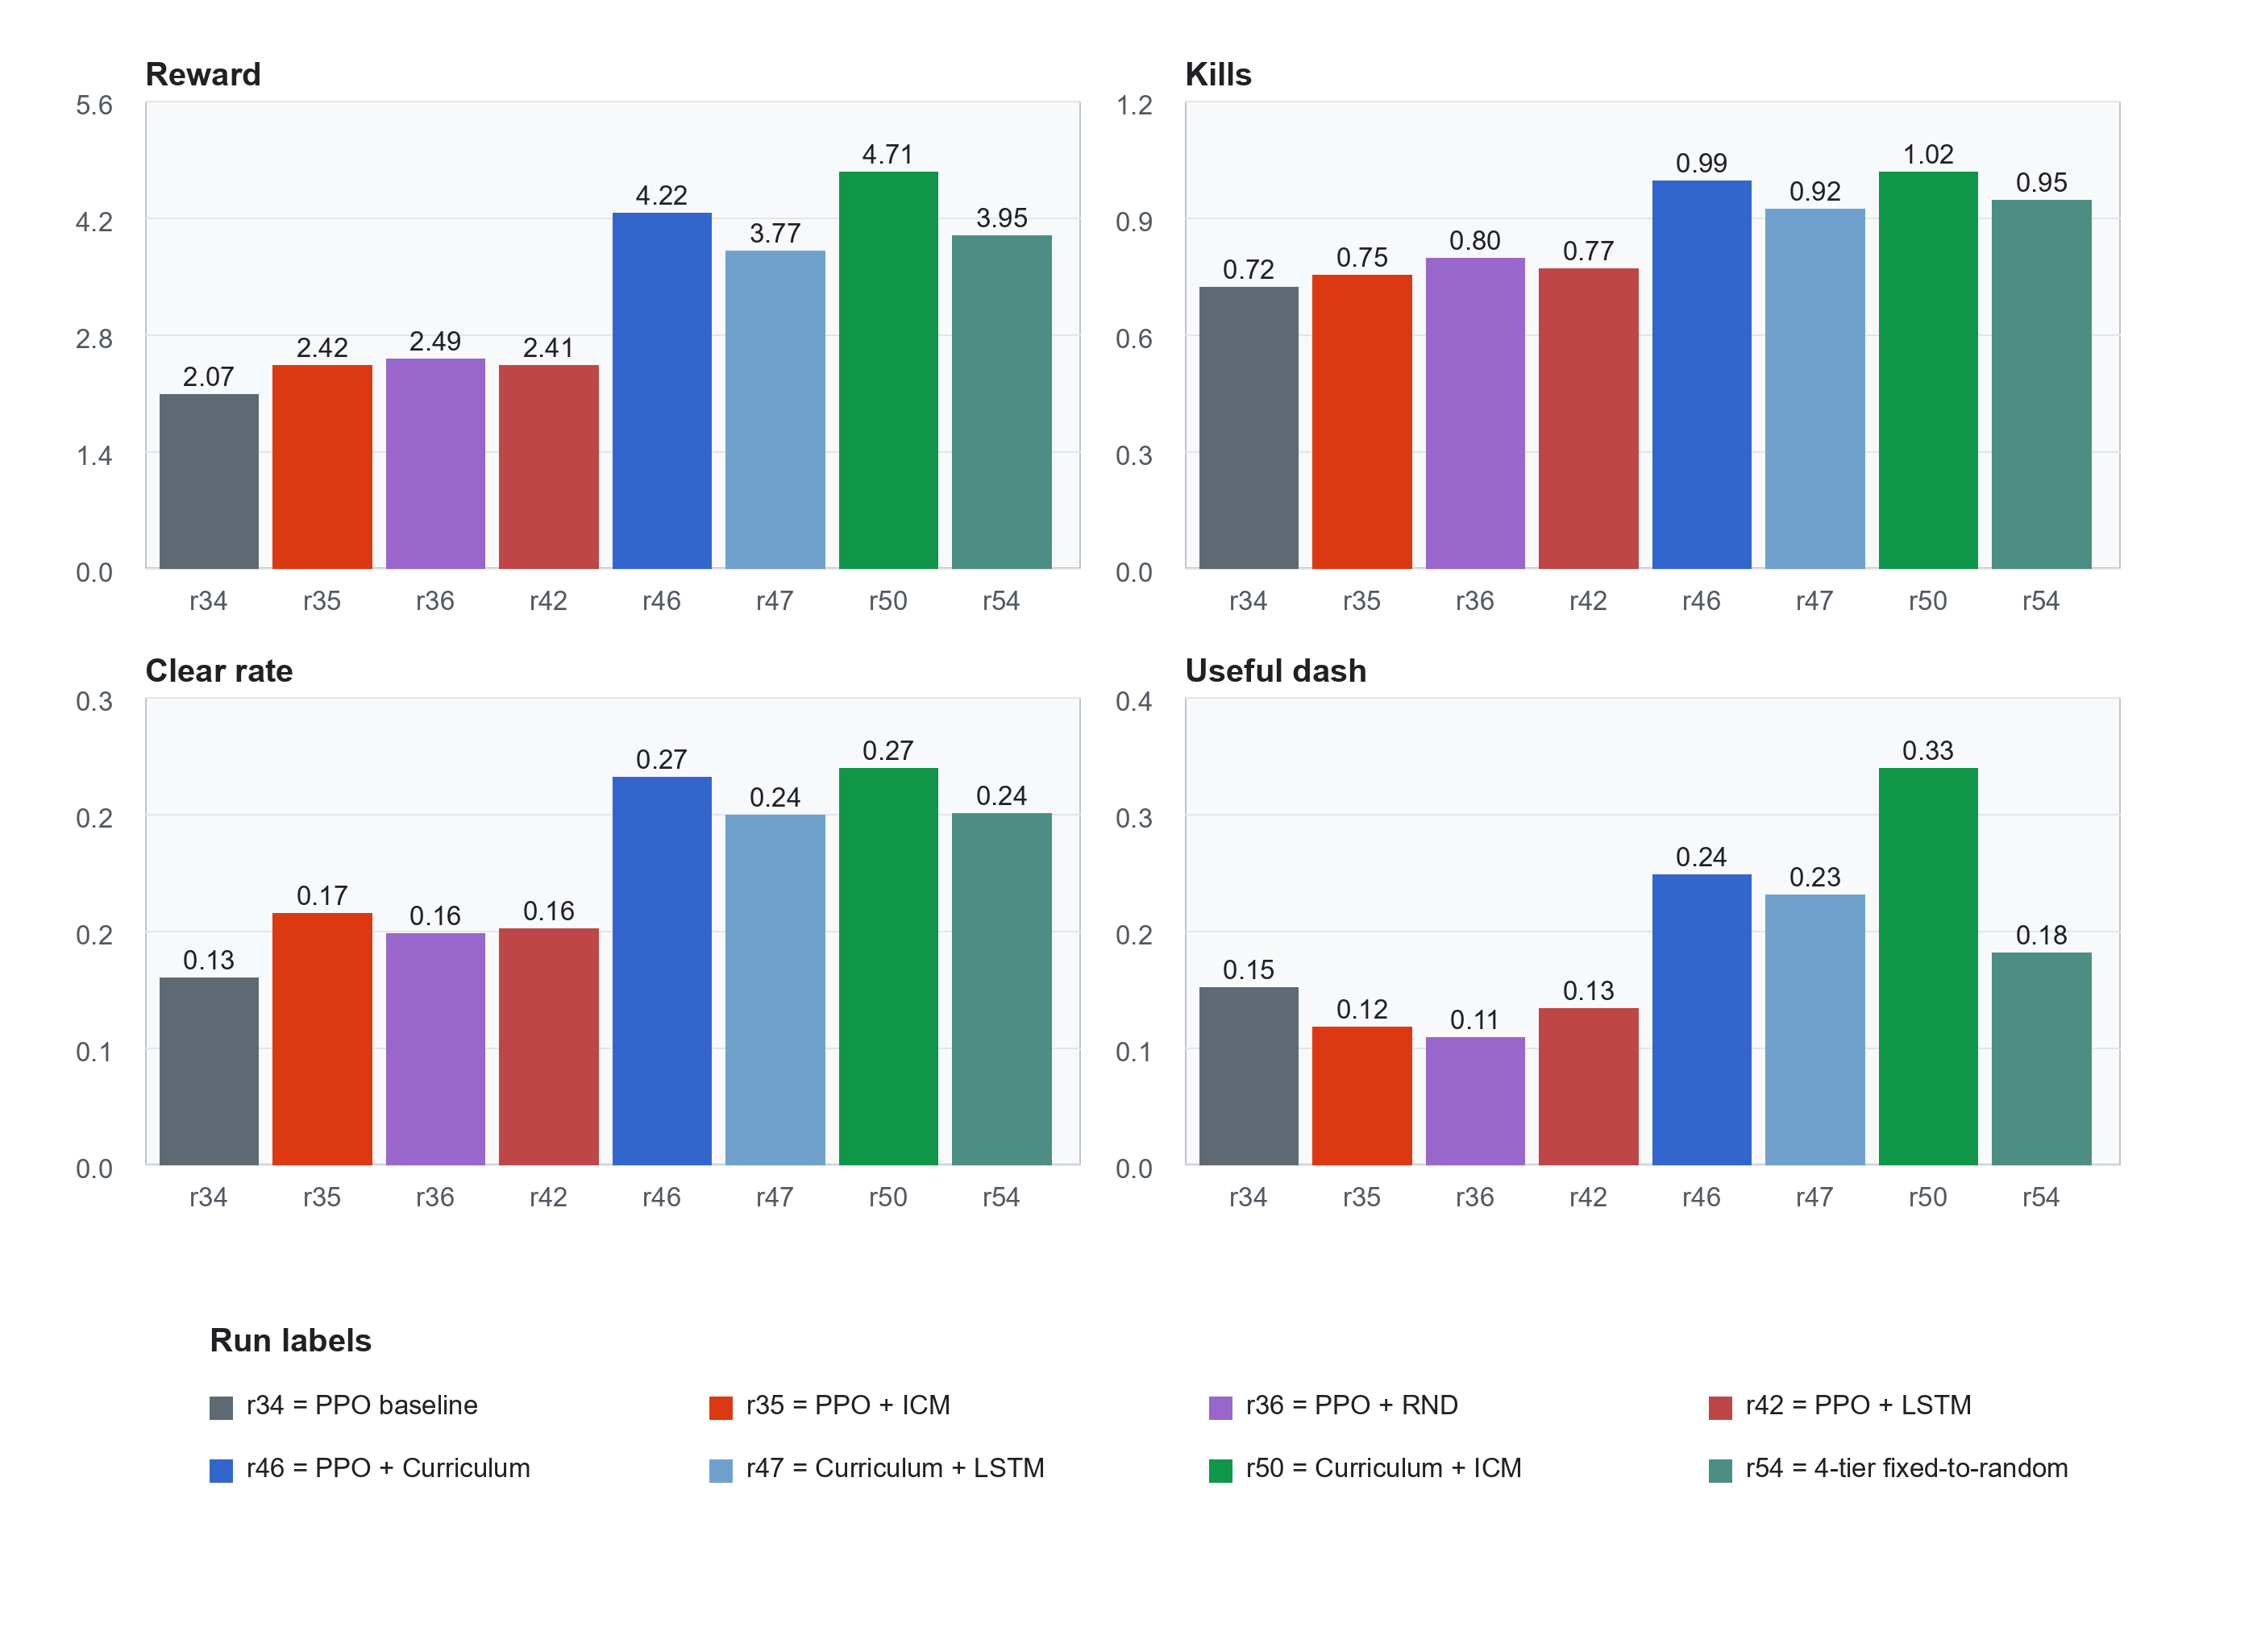
\includegraphics[width=0.98\textwidth]{figures/training/final_metrics_comparison.png}
    \caption{So sánh các chỉ số hành vi cuối run. Hình bổ sung cho Bảng~\ref{tab:run_metrics_main}: curriculum không chỉ tăng phần thưởng mà còn cải thiện số kẻ địch bị tiêu diệt, tỷ lệ dọn phòng và tỷ lệ dash hữu ích.}
    \label{fig:final_metrics_comparison}
\end{figure}

\section{Observation bottleneck -- run59: quan sát hỗ trợ BFS}

Sau các run ablation chính về kỹ thuật huấn luyện, đề tài thực hiện thêm run59 như một ablation mở rộng về biểu diễn quan sát. Mục tiêu của run này là kiểm tra một giả thuyết cụ thể: tác nhân có thể không thất bại chủ yếu vì không biết chiến đấu, mà vì biểu diễn quan sát 207 chiều chưa cung cấp đủ cấu trúc không gian để chính sách suy luận đường đi qua bản đồ có tường. Để kiểm tra giả thuyết này, run59 bổ sung ba chiều quan sát vào CombatAgent: hướng bước kế tiếp theo đường đi ngắn nhất tính bằng BFS và khoảng cách đường đi ngắn nhất đã chuẩn hóa tới kẻ địch còn sống gần nhất. Do đó, vector quan sát tăng từ 207 lên 210 chiều.

Run59 bổ sung yếu tố tìm đường vào quá trình học, do đó không thể so sánh trực tiếp với các run giữ nguyên quan sát 207 chiều. Chính sách vẫn dùng PPO và phải tự học các hành động di chuyển, ngắm, tấn công, dash; điểm khác biệt nằm ở việc phần điều hướng được hỗ trợ thêm bằng tín hiệu BFS. Nói cách khác, đây là biến thể \emph{BFS-assisted RL} hay \emph{path-informed observation} (quan sát có thông tin đường đi), nhằm đo tác động của tín hiệu đường đi đối với hiệu năng của tác nhân.

\begin{table}[H]
    \centering
    \small
    \caption{Kết quả cấu hình \emph{path-informed} sau bản cập nhật run61 ở mốc 1.0M bước}
    \label{tab:run59_bfs_assisted}
    \begin{tabular}{|p{4.1cm}|p{3.2cm}|p{6.4cm}|}
        \hline
        \textbf{Chỉ số} & \textbf{Giá trị cuối / vùng cuối} & \textbf{Diễn giải} \\
        \hline
        Phần thưởng tích lũy & 14.09 cuối run; tail gần cuối khoảng 14.77 & Cao hơn rõ so với các run chính, nhưng không so trực tiếp vì quan sát và định hình phần thưởng đã thay đổi. \\
        \hline
        Tỷ lệ dọn phòng & 0.727 cuối run; tail gần cuối khoảng 0.846 & Tác nhân dọn phòng ổn định hơn khi được cung cấp tín hiệu đường đi. \\
        \hline
        Số kẻ địch tiêu diệt/lượt & 1.55 cuối run; tail gần cuối khoảng 1.78 & Số kẻ địch bị tiêu diệt tăng, cho thấy khả năng điều hướng là một nút thắt thực tế của bài toán. \\
        \hline
        Entropy chính sách & Giảm từ khoảng 4.15 xuống 3.59; tail gần cuối khoảng 3.62 & Chính sách trở nên quyết đoán hơn so với các run bị plateau quanh 4.40 nat. \\
        \hline
        Phần thưởng nội tại (ICM) & Khoảng 0.005 ở cuối run & ICM không còn chi phối hành vi ở cuối run. \\
        \hline
        Số lần kẻ địch thoát kẹt & Tail gần cuối khoảng 3.07 mỗi episode & Môi trường vẫn còn nhiễu do kẻ địch bị kẹt hoặc cần phục hồi, nên kết quả cần được đọc kèm hạn chế thời gian chạy. \\
        \hline
    \end{tabular}
\end{table}

Bảng~\ref{tab:run59_bfs_assisted} cho thấy khi bổ sung tín hiệu đường đi ngắn nhất, các chỉ số hành vi tăng mạnh hơn: tỷ lệ dọn phòng đạt trên 0.8 ở vùng cuối, số kẻ địch bị tiêu diệt trung bình vượt 1.7 và entropy giảm sâu hơn so với plateau của các run 207 chiều. Đây là mức cải thiện đáng kể nhất trong toàn bộ quá trình thử nghiệm, vì nó không chỉ làm phần thưởng tăng mà còn cải thiện trực tiếp các chỉ số hành vi như tỷ lệ dọn phòng, số kẻ địch tiêu diệt và mức độ quyết đoán của chính sách. Có thể thấy nút thắt chính của môi trường không chỉ nằm ở thuật toán PPO hay cơ chế khám phá, mà còn ở biểu diễn không gian của quan sát. Khi tác nhân được cung cấp đặc trưng đường đi phù hợp hơn, chính sách có thể học hành vi tiếp cận và chiến đấu ổn định hơn. Các hướng tiếp theo nên tập trung vào local occupancy grid, graph/path feature học được, imitation learning cho điều hướng, hoặc thiết kế lại bản đồ/kẻ địch để giảm nhiễu từ các tình huống kẹt.

Run59 mang lại bước cải thiện lớn nhất về hiệu năng thực nghiệm, nhưng bản chất của cải thiện đến từ thay đổi biểu diễn quan sát chứ không chỉ từ thuật toán học. Kết quả không chứng minh tác nhân đã tự học tìm đường hoàn toàn; nó chỉ cho thấy khi được cung cấp đặc trưng đường đi phù hợp hơn, chính sách có thể học hành vi chiến đấu và tiếp cận mục tiêu ổn định hơn.

Bảng tổng hợp cho phép rút ra bốn nhận xét chính trong phạm vi thí nghiệm một seed. Trước hết, PPO baseline đạt hành vi hợp lý nhưng bị giới hạn ở mức phần thưởng khoảng 2.1--2.5. Tiếp đến, intrinsic motivation và LSTM chưa tạo cải thiện lớn khi chạy độc lập. Đáng chú ý hơn, curriculum learning là yếu tố nổi bật nhất; khi kết hợp thêm ICM, phần thưởng Hard tăng lên 4.369 nhưng inverse loss vẫn cao. Cuối cùng, entropy plateau vẫn tồn tại trong nhóm ablation chính 207 chiều. Ở run62, khi kết hợp quan sát lưới cục bộ, curriculum 4 bậc, ICM và huấn luyện đến 33.45M bước, entropy giảm xuống 3.099 nat và clear\_rate đạt 0.626. Tuy nhiên, do run62 thay đổi nhiều yếu tố đồng thời, kết quả này được xem là bằng chứng thăm dò thay vì ablation đơn biến.

\section{Observation bottleneck -- run62: local grid end-to-end}

Sau khi run59/61 xác định biểu diễn không gian và tín hiệu điều hướng là yếu tố đột phá, đề tài tiến hành run62 với cấu hình kết hợp. Quan sát chuyển sang lưới cục bộ để mở rộng đặc trưng không gian; curriculum được nâng lên 4 bậc (EasyFixed $\rightarrow$ MediumFixed $\rightarrow$ HardFixed $\rightarrow$ HardRandom); ICM bật với strength 0.001; tham số \texttt{aggressive\_seek} luôn bật để kẻ địch truy đuổi tích cực hơn. Run chạy trên 8 môi trường song song trong hai session liên tiếp do giới hạn tài nguyên, tổng cộng đạt \textbf{33.45M bước} -- 24.25M bước ở session đầu, thêm 9.2M bước ở session sau với trọng số khởi tạo từ checkpoint 24.25M.

\begin{figure}[H]
    \centering
    
\includegraphics[width=0.98\textwidth]{figures/training/run62_merged_overview.png}
    \caption{Tổng quan quá trình huấn luyện 33.45M bước: phần thưởng, tỷ lệ dọn phòng, số kẻ địch tiêu diệt và entropy. Đường kẻ dọc đánh dấu điểm bắt đầu session thứ hai (24.25M bước).}
    \label{fig:run62_merged_overview}
\end{figure}

Sau 33.45M bước, phần thưởng tail-50 đạt 14.105 (đỉnh 18.673), số kẻ địch tiêu diệt tail-50 đạt 1.530, tỷ lệ dọn phòng tail-50 đạt 0.626 và tỷ lệ dash hữu ích đạt 0.400. Tỷ lệ dọn phòng 0.626 nằm giữa run46 curriculum baseline (0.267) và run61 BFS-assisted (0.846), nhưng đáng chú ý là run này không cài cứng BFS mà chỉ dùng quan sát lưới cục bộ để tác nhân tự học không gian từ dữ liệu, cho thấy lưới cục bộ có thể tiệm cận BFS khi quy mô huấn luyện đủ lớn.

Điểm quan trọng nhất là entropy giảm bền vững từ vùng plateau 4.40 nat của các ablation 1--3M bước xuống còn 3.099 tail-50, tức thấp hơn 1.3 nat so với plateau cũ. Đây là lần đầu tiên entropy plateau bị phá vỡ hoàn toàn trong suốt quá trình huấn luyện; tuy nhiên vì run62 thay đổi nhiều yếu tố đồng thời, chưa thể xác định lưới cục bộ là yếu tố duy nhất quyết định kết quả này.

\begin{figure}[H]
    \centering
    
\includegraphics[width=0.98\textwidth]{figures/training/run62_merged_entropy.png}
    \caption{Entropy chính sách giảm xuống dưới plateau 4.40 nat và duy trì bền vững. Vùng tô màu biểu thị khoảng entropy nằm dưới plateau cũ.}
    \label{fig:run62_merged_entropy}
\end{figure}

\begin{table}[H]
    \centering
    \small
    \setlength{\tabcolsep}{4pt}
    \renewcommand{\arraystretch}{1.2}
    \caption{Chỉ số hành vi chính của run62 (33.45M bước gộp)}
    \label{tab:run62_metrics}
    \begin{tabular}{|p{4.5cm}|c|c|c|c|c|c|c|}
        \hline
        \textbf{Thiết lập} & \textbf{Step} & \textbf{Reward} & \textbf{Clear} & \textbf{Kills} & \textbf{Dmg+} & \textbf{Ent} & \textbf{V-est} \\
        \hline
        LocalGrid + Aggressive + ICM + 4-tier curriculum & 33.45M & 14.105 & 0.626 & 1.530 & 47.780 & 3.099 & 2.455 \\
        \hline
    \end{tabular}
\end{table}

Run62 đem lại hai kết luận. Thứ nhất, entropy plateau 4.40 nat quan sát ở các ablation 1--3M bước với quan sát 207 chiều không phải giới hạn cứng của PPO hay action space, mà là hệ quả của số bước huấn luyện chưa đủ kết hợp với quan sát thiếu đặc trưng không gian; khi tất cả các yếu tố trong cấu hình run62 được kết hợp, entropy giảm bền vững. Thứ hai, khi lưới cục bộ được huấn luyện đến 33.45M bước, tác nhân có thể đạt tỷ lệ dọn phòng tiệm cận BFS-assisted mà không cần cài cứng cơ chế tìm đường -- mở ra hướng học hoàn toàn end-to-end cho bài toán điều hướng trong môi trường có tường.
